% !TEX root = ../thesis.tex

\chapter{Syntetická časť}
\label{methodology}
V tejto časti si prejdeme konceptuálny návrh riešenia a bližšie sa pozrieme na metódy a hodnoty, ktoré budú potrebné pri jednotlivých fázach z návrhu riešenia, a na finálnu tvorbu prototypu 
\section{Konceptuálny návrh riešenia}

 \begin{figure}[h!]
	
	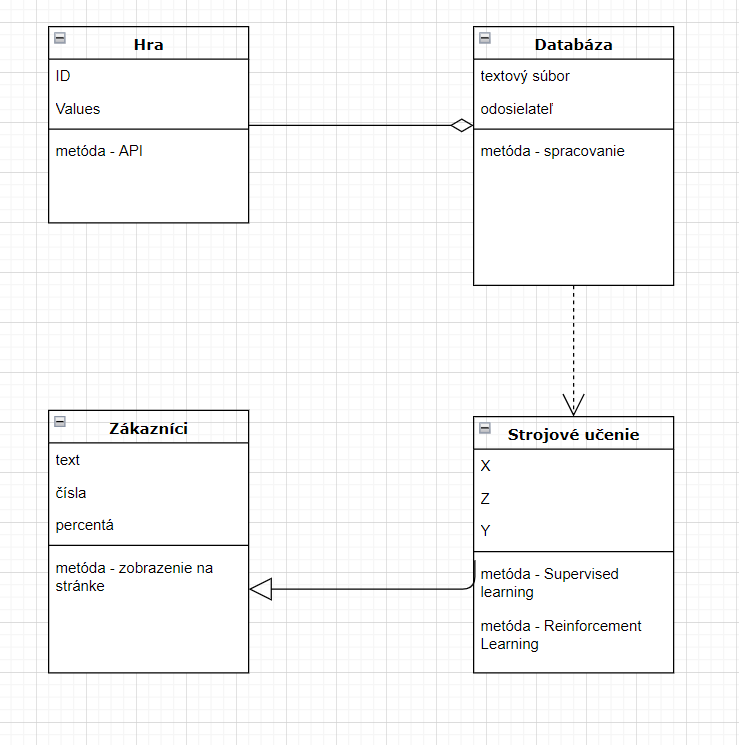
\includegraphics[width=.9\textwidth]{figures/navrhriesenia}
	\centering
	\caption{ Konceptuálny návrh riešenia \label{koncept}}
	
\end{figure}

Ako môžeme vidieť na obrázku \ref{koncept}, na návrh riešenia treba spracovať 4 fázy : 

\begin{enumerate}
	\item Prevziať potrebné dáta z hier cez API
	\item Spracovať ich do čitateľnej verzie pre umelú inteligenciu
	\item Použiť dáta na natrénovanie modelu
	\item Spracovať výsledky do čitateľnej formy pre zákazníkov
\end{enumerate}

\section{Prevzatie dát z developer Riotgames cez API}

\section{Opis metód}
Hlavné metódy pri učení nášho modelu.
\subsection{Supervised learning}
Podkategória umelej inteligencie, ktorá používa daný dataset na natrénovanie modelu.

\subsection{Reinforcement learning}
Časť umelej inteligencie, pri ktorej sa sledujú kroky inteligentných agentov na maximalizáciu efektívnosti dosiahnutia cieľa.

